\section{Descripción del problema}

%%%%%%%%%%%%%%%%%%%%%%%%%%%%%%%%%%%%%%%%%%%%%%%%%%%%%%%%%%%%%%%%%%%%%%%%%
%%%%%%%%%%%%%%%%%%%%%%%%%%%%%%%%%%%%%%%%%%%%%%%%%%%%%%%%%%%%%%%%%%%%%%%%%
%%%%%%%%%%%%%%%%%%%%%%%%%%%%%%%%%%%%%%%%%%%%%%%%%%%%%%%%%%%%%%%%%%%%%%%%%

\subsection{Descripción del problema}

\begin{frame}

    \begin{figure}
        \centering
        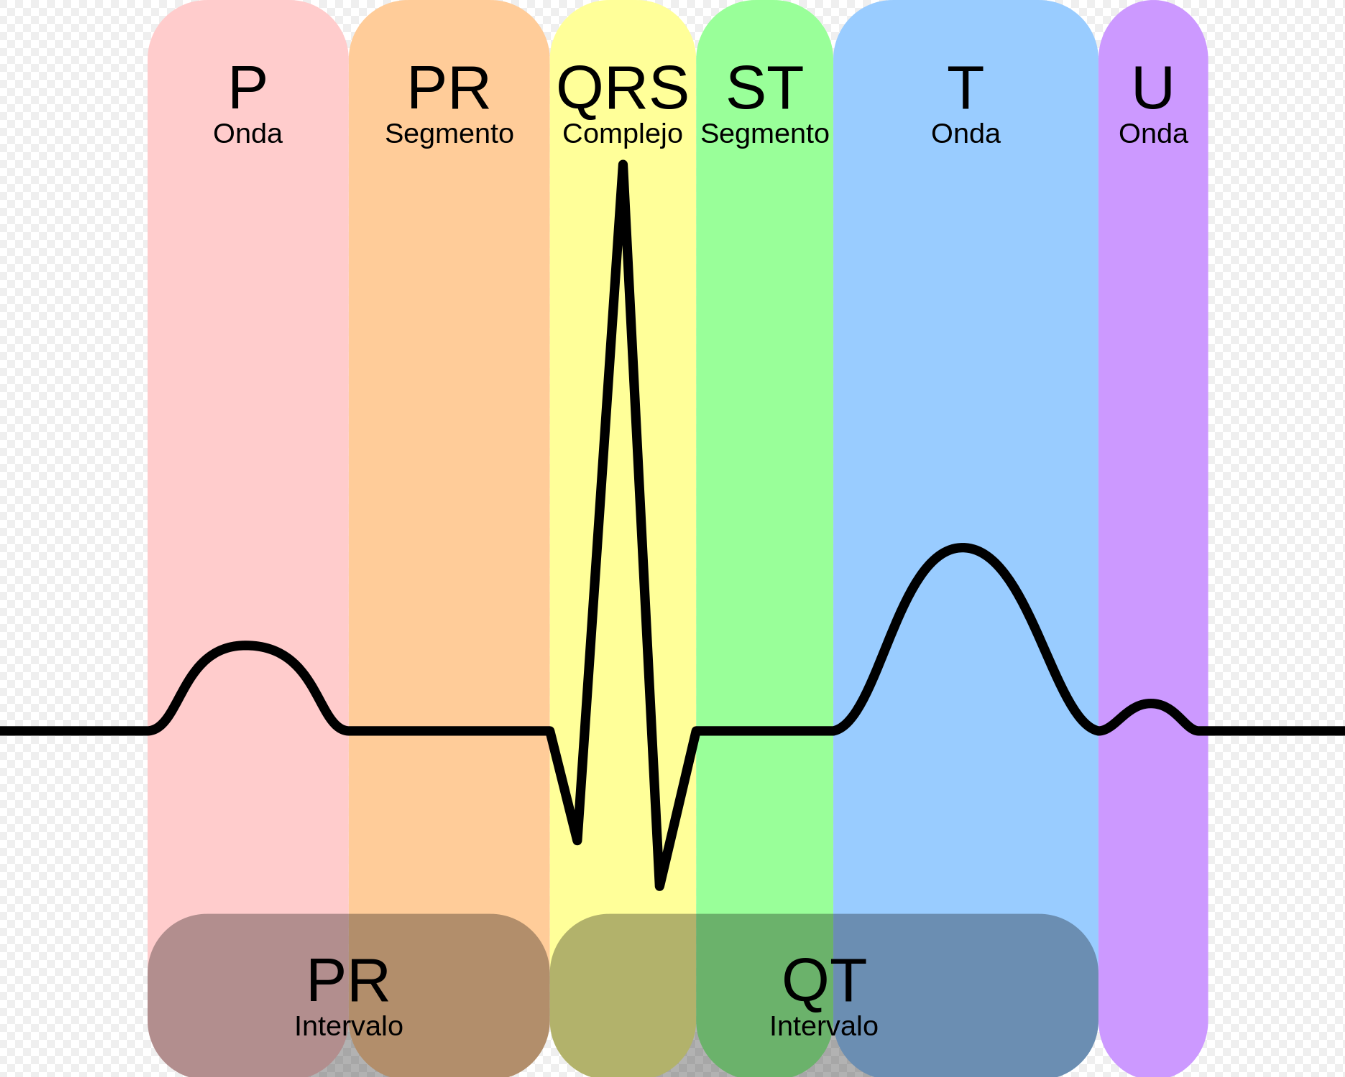
\includegraphics[scale=0.1]{Images/ECG_2.png}
    \end{figure}
    \begin{itemize}
        \pause
        \item Problema de clasificación de señales obtenidas por ECG.
        \pause
        \item Principal objetivo: Discernir entre ritmos normales, FA y otras patologías.
        \pause
        \item Existen dos enfoques para abordar esto.
        \pause
        \begin{itemize}
            \item Enfoque tradicional: Extracción de características a mano
            \item Enfoque moderno: {\color{TurkishRose} \textit{Técnicas de aprendizaje profundo}}
        \end{itemize}
    \end{itemize}
\end{frame}

%%%%%%%%%%%%%%%%%%%%%%%%%%%%%%%%%%%%%%%%%%%%%%%%%%%%%%%%%%%%%%%%%%%%%%%%%
%%%%%%%%%%%%%%%%%%%%%%%%%%%%%%%%%%%%%%%%%%%%%%%%%%%%%%%%%%%%%%%%%%%%%%%%%
\subsection{Base de datos}

\begin{frame}
\begin{overprint}
    \onslide<1>
        \begin{itemize}
            \item PhysioNet/CinC, competición 2017.
            \item 4 clases
        \end{itemize}
        
    \onslide<2>
        \begin{itemize}
            \item PhysioNet/CinC, competición 2017.
            \item 4 clases: 
                \begin{itemize}
                    \item Ritmo sinusal normal
                \end{itemize}
        \end{itemize}
        
        \begin{figure}
            \centering
            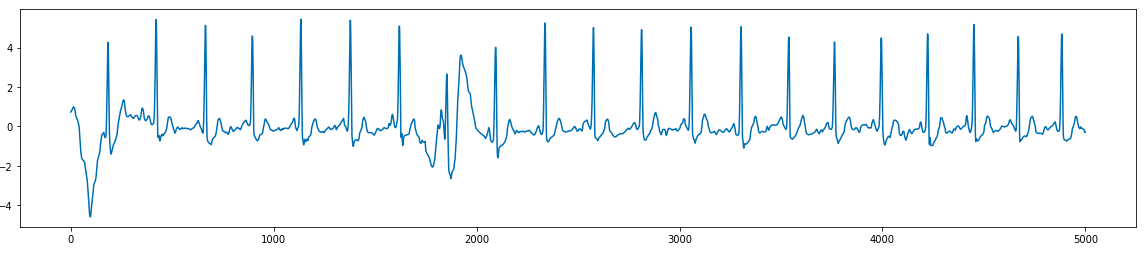
\includegraphics[keepaspectratio=true,height=0.25\paperheight]{Images/Normal.png}
        \end{figure}
    
    \onslide<3>
        \begin{itemize}
            \item PhysioNet/CinC, competición 2017.
            \item 4 clases: 
                \begin{itemize}
                    \item Ritmo sinusal normal
                    \item Fibrilación auricular
                \end{itemize}
        \end{itemize}
        
        \begin{figure}
            \centering
            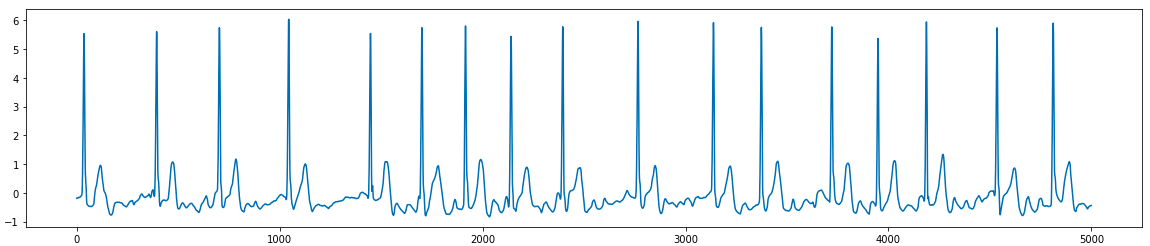
\includegraphics[keepaspectratio=true,height=0.25\paperheight]{Images/FA.png}
        \end{figure}
    
    \onslide<4>
        \begin{itemize}
            \item PhysioNet/CinC, competición 2017.
            \item 4 clases: 
                \begin{itemize}
                    \item Ritmo sinusal normal
                    \item Fibrilación auricular
                    \item Otro (Otra patología)
                \end{itemize}
        \end{itemize}
        
        \begin{figure}
            \centering
            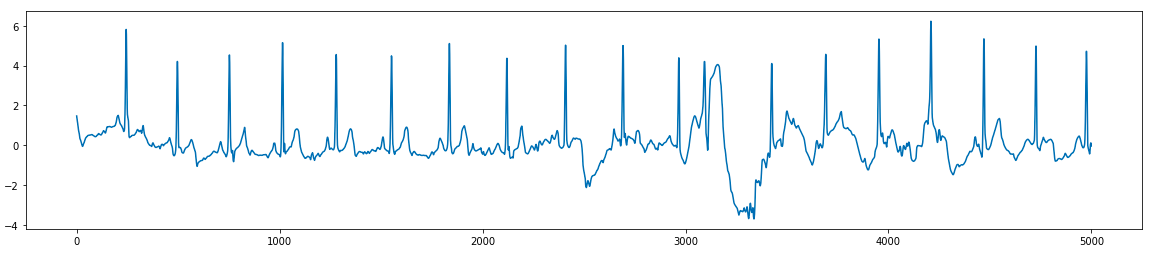
\includegraphics[keepaspectratio=true,height=0.25\paperheight]{Images/Other.png}
        \end{figure}
        
        
    \onslide<5>
        \begin{itemize}
            \item PhysioNet/CinC, competición 2017.
            \item 4 clases: 
                \begin{itemize}
                    \item Ritmo sinusal normal
                    \item Fibrilación auricular
                    \item Otro (Otra patología)
                    \item Ritmo demasiado ruidoso
                \end{itemize}
        \end{itemize}
        
        \begin{figure}
            \centering
            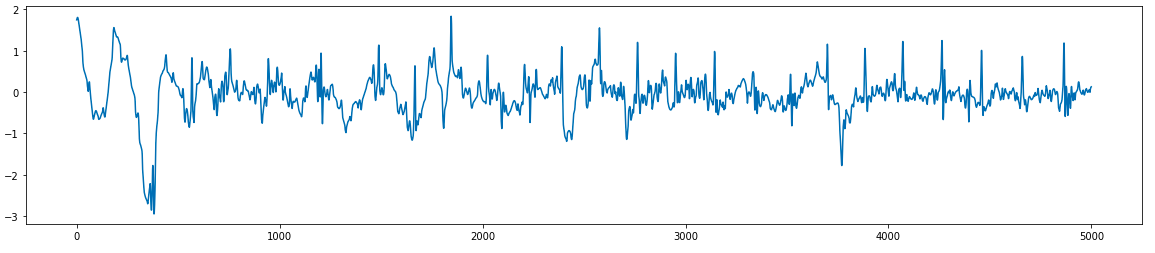
\includegraphics[keepaspectratio=true,height=0.25\paperheight]{Images/noise.png}
        \end{figure}
        
    \onslide<6>
        \begin{itemize}
            \item PhysioNet/CinC, competición 2017.
            \item 4 clases: 
                \begin{itemize}
                    \item Ritmo sinusal normal
                    \item Fibrilación auricular
                    \item Otro (Otra patología)
                    \item Ritmo demasiado ruidoso
                \end{itemize}
            \item Fuerte Desbalanceo entre clases
        \end{itemize}
        
        \begin{table}[htbp]
            \begin{center}
            \resizebox{0.95\columnwidth}{!}{
            \begin{tabular}{|l|r|r|r|r|r|r|}
            \hline
            \textbf{Tipo} & \multicolumn{1}{l|}{\textbf{Cantidad}} & \multicolumn{1}{l|}{\textbf{Media}} & \multicolumn{1}{l|}{\textbf{SD}} & \multicolumn{1}{l|}{\textbf{Max}} & \multicolumn{1}{l|}{\textbf{Mediana}} & \multicolumn{1}{l|}{\textbf{Min}} \\ \hline
            \textbf{Normal} & 5154 & 31,9 & 10 & 61 & 30 & 9 \\ \hline
            \textbf{AF} & 771 & 31,6 & 12,5 & 60 & 30 & 10 \\ \hline
            \textbf{Otro Ritmo} & 2557 & 34,1 & 11,8 & 60,9 & 30 & 9,1 \\ \hline
            \textbf{Ruido} & 46 & 27,1 & 9 & 60 & 30 & 10,2 \\ \hline
            \textbf{Total} & 8528 & 32,5 & 10,9 & 61 & 30 & 9 \\ \hline
            \end{tabular}}
            \end{center}
            \caption{Datos del conjunto de entrenamiento}
            \label{table:BD}
        \end{table}
\end{overprint}
\end{frame}



%%%%%%%%%%%%%%%%%%%%%%%%%%%%%%%%%%%%%%%%%%%%%%%%%%%%%%%%%%%%%%%%%%%%%%%%%
%%%%%%%%%%%%%%%%%%%%%%%%%%%%%%%%%%%%%%%%%%%%%%%%%%%%%%%%%%%%%%%%%%%%%%%%%

\subsection{Desarrollo de los modelos}

\begin{frame}{Mejores modelos de la competición}

    {\vspace{-1.5cm} \textit{Modus operandis}: Extracción de características de manera manual y posterior clasificación.} \\
    \vspace{1 cm}
    Modelos:
    \pause 
    \begin{itemize}
        \item Clasificador binario en cascada
        \pause
        \item EnCaSe
        \pause
        \item Marco de interpretación abductivo
        \pause 
        \item Clasificador basado en Random Forest
    \end{itemize}
    
\end{frame} 

%%%%%%%%%%%%%%%%%%%%%%%%%%%%%%%%%%%%%%%%%%%%%%%%%%%%%%%%%%%%%%%%%%%%%%%%%

\begin{frame}{Modelos propuestos de la literatura}
    \begin{overprint}
        
        \onslide<1>
            \begin{center}
                {\color{TurkishRose} \textbf{\textit{OhShuLi}}}
            \end{center}
            \begin{figure}
                \centering
                \vspace{-1cm}
                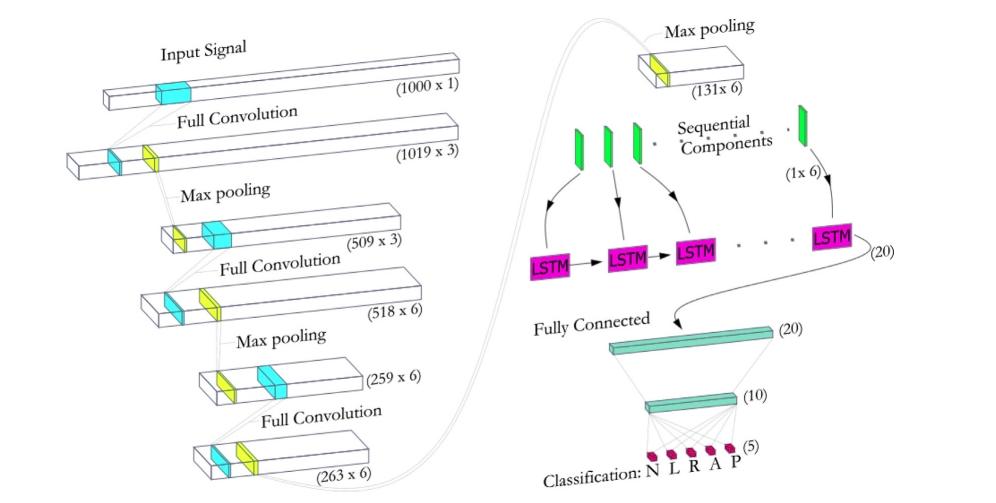
\includegraphics[keepaspectratio=true,height=0.9\paperheight,width=0.95\paperwidth]{Images/ohshuli1.png}
            \end{figure}
            
        \onslide<2>
            \begin{center}
                {\color{TurkishRose} \textbf{\textit{ChenChen}}}
            \end{center}
            \begin{figure}
                \centering
                \vspace{-0.3cm}
                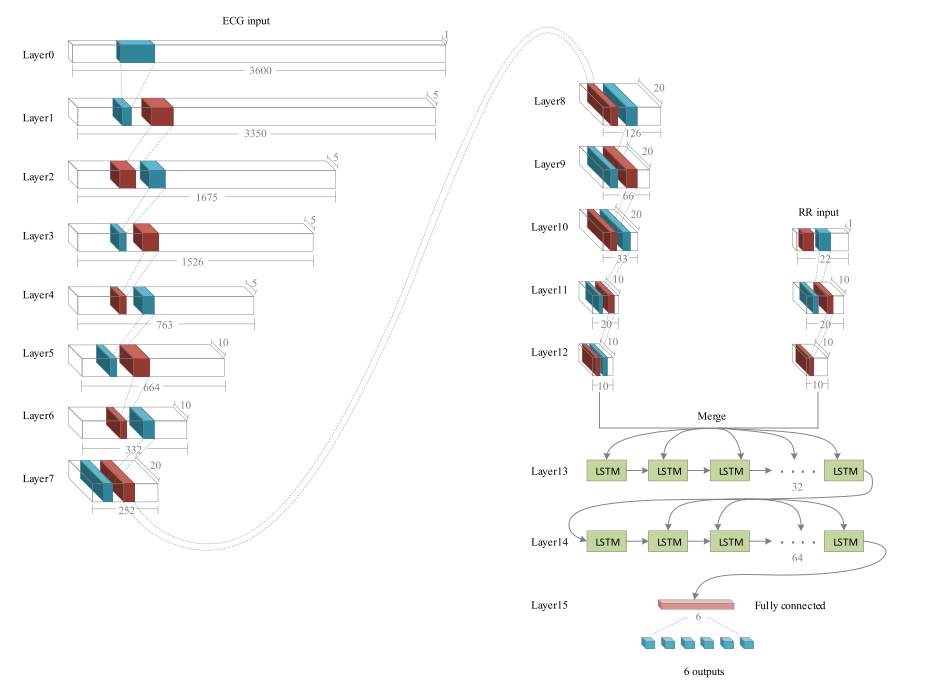
\includegraphics[keepaspectratio=true,height=0.65\paperheight,width=0.8\paperwidth]{Images/chenchen1.png}
            \end{figure}
        
        \onslide<3>
            \begin{center}
                {\color{TurkishRose} \textbf{\textit{GaoJunLi}}}
            \end{center}
            \begin{figure}
                \centering
                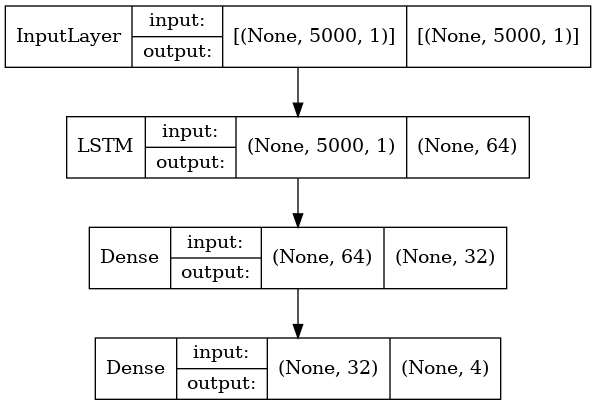
\includegraphics[keepaspectratio=true,height=0.6\paperheight,width=0.7\paperwidth]{Images/GaoJunLin.png}
            \end{figure}
    \end{overprint}
\end{frame} 

%%%%%%%%%%%%%%%%%%%%%%%%%%%%%%%%%%%%%%%%%%%%%%%%%%%%%%%%%%%%%%%%%%%%%%%%%

\begin{frame}{Modelos propios}
\begin{overprint}
    \onslide<1>
        \begin{center}
            {\color{TurkishRose} \textbf{\textit{CNN}}}
        \end{center}
        
        \begin{figure}
            \centering
            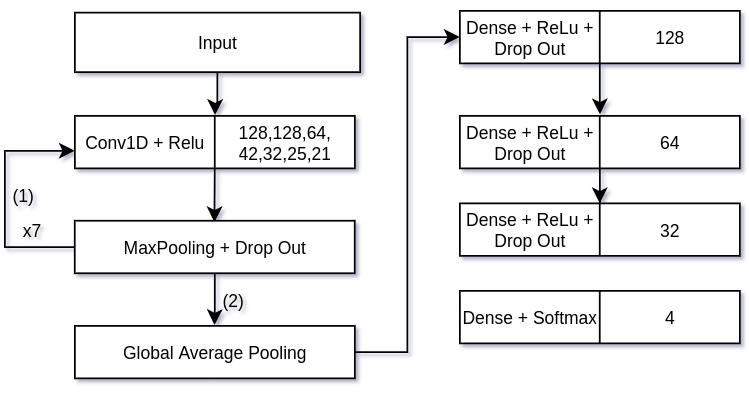
\includegraphics[keepaspectratio=true,height=0.65\paperheight,width=0.8\paperwidth]{Images/cnn diagram.png}
        \end{figure}
        
    \onslide<2>
        \begin{center}
            {\color{TurkishRose} \textbf{\textit{LSTM}}}
        \end{center}    
        
        \begin{figure}
            \centering
            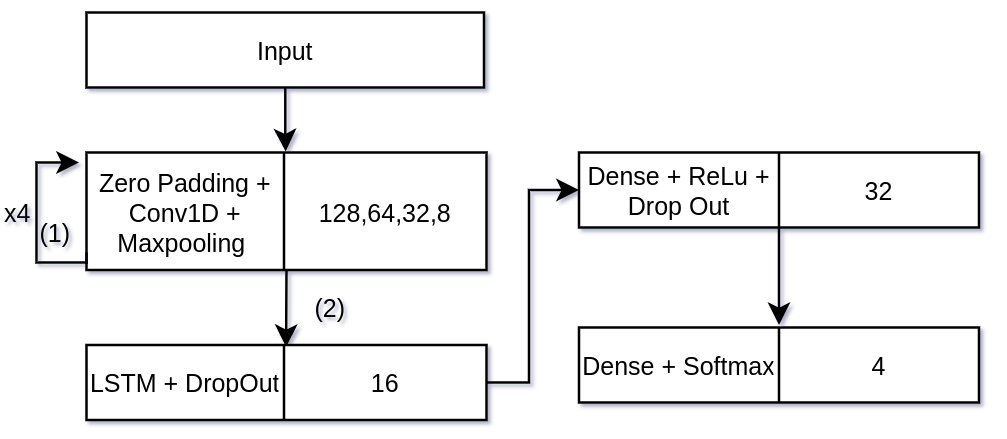
\includegraphics[keepaspectratio=true,height=0.65\paperheight,width=0.8\paperwidth]{Images/LSTM diagram.png}
        \end{figure}

            
    \onslide<3>
        \begin{center}
            {\color{TurkishRose} \textbf{\textit{GRU}}}
        \end{center}

        \begin{figure}
            \centering
            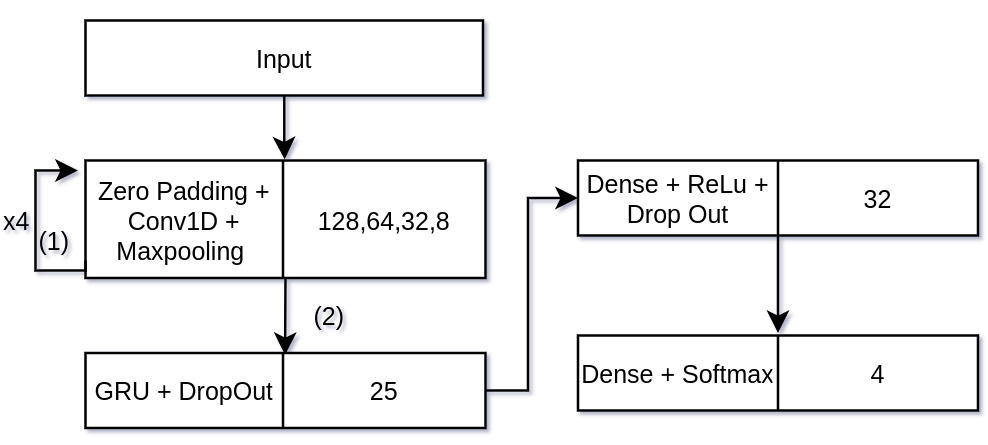
\includegraphics[keepaspectratio=true,height=0.65\paperheight,width=0.8\paperwidth]{Images/GRU diagram.png}
        \end{figure}
\end{overprint}
\end{frame}



%%%%%%%%%%%%%%%%%%%%%%%%%%%%%%%%%%%%%%%%%%%%%%%%%%%%%%%%%%%%%%%%%%%%%%%%%
%%%%%%%%%%%%%%%%%%%%%%%%%%%%%%%%%%%%%%%%%%%%%%%%%%%%%%%%%%%%%%%%%%%%%%%%%

\subsection{Métrica}

\begin{frame}{$F_1$ score}
    \begin{overprint}

        \onslide<1>
        
            \begin{figure}[H]
                \centering
                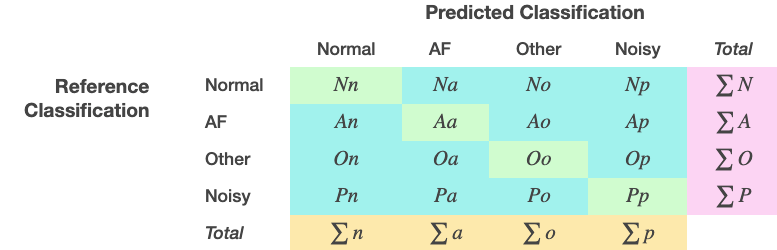
\includegraphics[width=\textwidth]{Images/metrica_2.png}
            \end{figure}
            
            \begin{columns}
                \column{0.4\textwidth}\centering
                \begin{itemize}
                    \item Ritmo normal:
                    \begin{equation*}
                        F_{1n} = \frac{2 Nn}{\sum_{N} + \sum_{n}}
                    \end{equation*}
                    \item Ritmo AF:
                    \begin{equation*}
                        F_{1a} = \frac{2 Aa}{\sum_{N} + \sum_{n}}
                    \end{equation*}
                 \end{itemize}
                
                \column{0.6\textwidth}\centering
                \begin{itemize}
                    \item Otro ritmo:
                    \begin{equation*}
                        F_{1o} = \frac{2 Oo}{\sum_{O} + \sum_{o}}
                    \end{equation*}
                    \item Ruido:
                    \begin{equation*}
                        F_{1p} = \frac{2 Pp}{\sum_{P} + \sum_{p}}
                    \end{equation*}
        
                \end{itemize}
                \end{columns}
                
                
        \onslide<2>
            \begin{figure}[H]
                \centering
                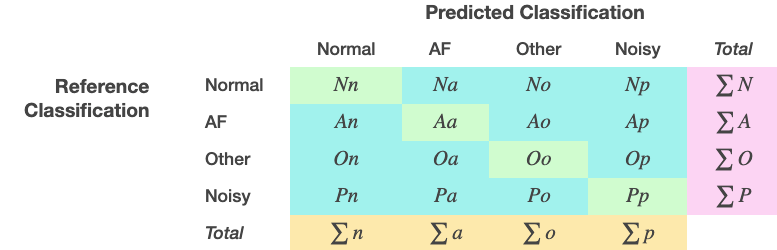
\includegraphics[width=\textwidth]{Images/metrica_2.png}
            \end{figure}
        \begin{itemize}
            \item $F_1:$     
            \begin{equation*}
                F_1 = \frac{F_{1n} + F_{1a} + F_{1o} + F_{1p}}{4}
            \end{equation*}
        \end{itemize}

    \end{overprint}
\end{frame}

